\chapter{Finite Element Modeling}
\label{chap:FEM}

This chapter outlines the development of the finite element model of the UBX metro and the simulation setup. First, in section \ref{section:geometry}, the design of the model geometry and the mesh of the model are shown. Consecutively, section \ref{section:boundary_conditions} describes the incorporation of boundary conditions into the finite element model. Finally, in section \ref{section:parametric_study}, a parametric study is carried out to investigate the influence of different simulation parameters on the solution of the initial finite element model. All these simulations are executed with the acoustics module of the open-source FEM software openCFS \cite{opencfs}.


\section{Geometry and mesh}
\label{section:geometry}

Due to the large dimension of the car body, the computation of the complete model would be too extensive. Hence, the simulation model constitutes of the front bogie part only. The latter has been marked through a red box in fig. \ref{fig:red_box}. Furthermore, the outer pressure field measurement described in sec. \ref{sec:pressure_field_measurement} has been taken from the same area.


\begin{figure}[H]
	\centering
	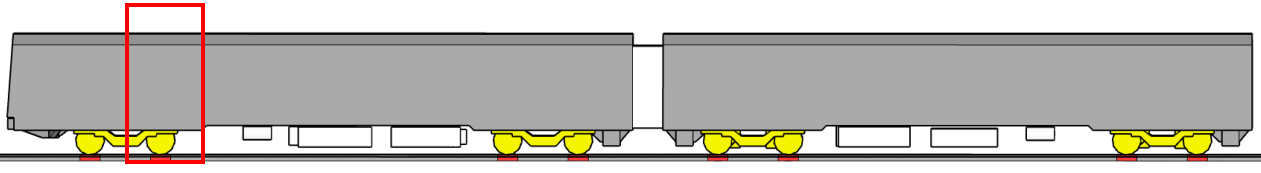
\includegraphics[width=\textwidth]{fig/chap4/geometry/model_area.png}
	\caption{Side view of UBX, red box indicates the modeling area}
	\label{fig:red_box}
\end{figure}

In order to reduce computational effort, the symmetry of the model is exploited. The quarter model is depicted in fig. \ref{fig:fourth_model}, whereas the equivalent model, namely the full model, is shown in fig. \ref{fig:full_model}. Both models are shown for more comprehensive illustration of the modeled underfloor components, but only the quarter model has been used in the simulation. For simplification of the geometry design, exclusively the most essential components have been included in the model. Starting with the squared car body (dark green), the bogie (purple), the wheel (pink), the air suspension (gray) and ending with the omnidirectional loudspeaker (bright green). This respective component has been placed underneath the car floor, between bogie and the wheel axle and is represented through a sphere with $35\,\text{cm}$ diameter.


\begin{figure}[H]
	\centering
	\begin{subfigure}[b]{0.4\textwidth}
		\centering
		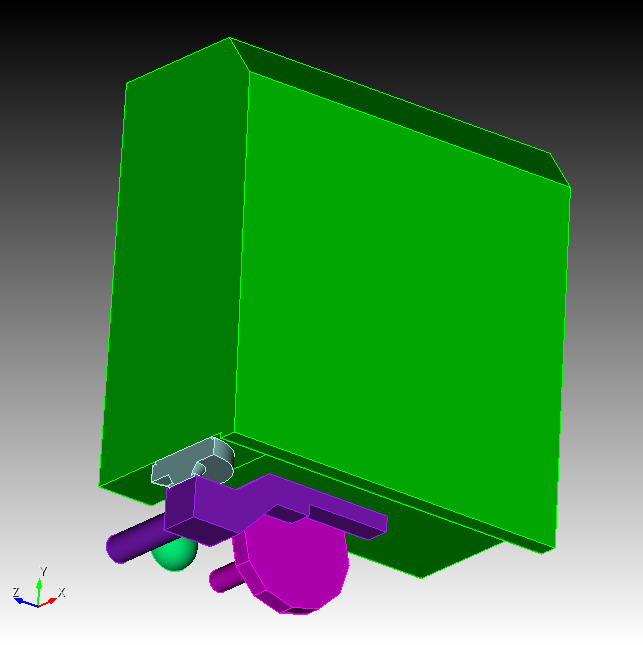
\includegraphics[width=0.9\linewidth]{fig/chap4/geometry/one_fourth_model.png}
		\caption{quarter model}
		\label{fig:fourth_model}
	\end{subfigure}
	\hfill
	\begin{subfigure}[b]{0.4\textwidth}
		\centering
		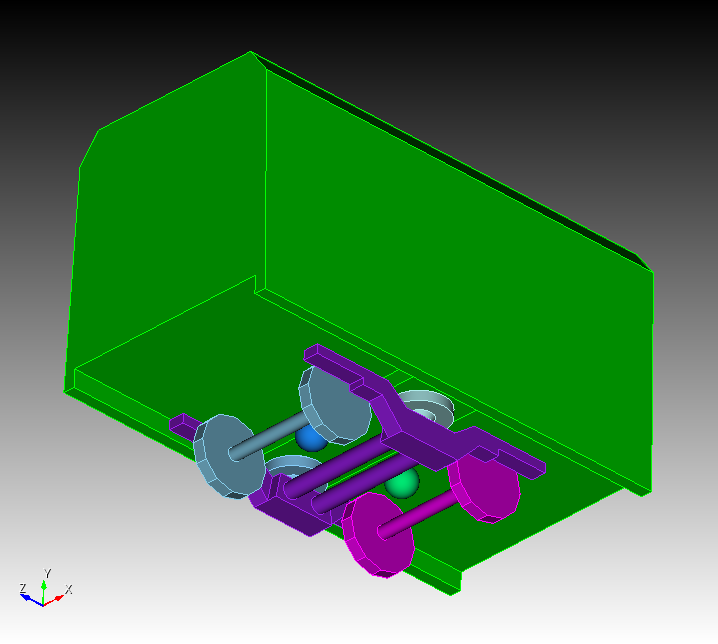
\includegraphics[width=\linewidth]{fig/chap4/geometry/initial_model_2.png}
		\caption{full model}
		\label{fig:full_model}
	\end{subfigure}
	\caption{Geometry of model}
\end{figure}

The quarter model has been cut out from an acoustic region, surrounded by a perfectly matched layer to simulate the free field condition.

is surrounded by pml to model the open infinite domain

A mesh has been created from the 3d model.

\begin{figure}[H]
	\centering
	\begin{subfigure}[b]{0.45\textwidth}
		\centering
		\includegraphics[width=\linewidth]{fig/chap4/mesh/propagation_domain.png}
		\caption{Propagation region (green) surrounded by a PML (gray)}
		\label{fig:propagation_domain}
	\end{subfigure}
	\hfill
	\begin{subfigure}[b]{0.45\textwidth}
		\centering
		\includegraphics[width=\linewidth]{fig/chap4/mesh/mesh1.png}
		\caption{mesh of the acoustic region}
		\label{fig:mesh_model}
	\end{subfigure}
	\caption{Acoustic region}
\end{figure}




\subsection*{Determination of simulation domain}

The goal of this section is to find an appropriate propagation domain size to achieve sufficient numerical accuracy while keeping the computational effort low. For the variation, the length and height of the propagation domain are kept constant while only the width of the domain is varied.

\begin{figure}[H]
	\centering
	\begin{subfigure}[b]{0.45\textwidth}
		\centering
		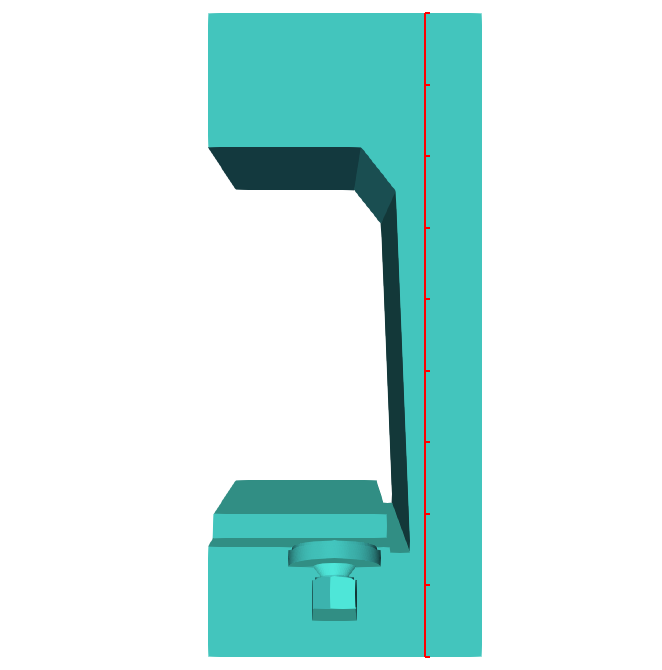
\includegraphics[width=\linewidth]{fig/chap4/simulation_domain/0pt5m.png}
		\caption{0.5 m}
	\end{subfigure}
	\hfill
	\begin{subfigure}[b]{0.45\textwidth}
		\centering
		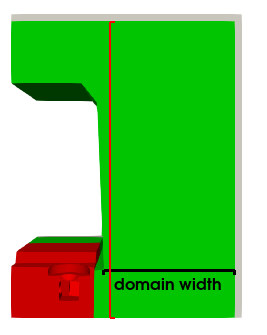
\includegraphics[width=\linewidth]{fig/chap4/simulation_domain/2m.png}
		\caption{2 m}
	\end{subfigure}
	\caption{Models with different simulation domain size}
	\label{fig:domain_size_variation}
\end{figure}

The compared simulation domain size are 0.2 m, 0.5 m, 1 m, 1.5 m and 2m. For each setup, the pressure is evaluated at 0.1 m away from the vehicle along the height direction, and the result is compared to a , the model with 2 m domain size will be used as reference. Fig. \ref{fig:domain_size_variation} shows the model with 0.5 m domain size and the reference model with 2 m domain size. The evaluation position is marked by the red line.


\subsection*{Computational Effort}
The aim of this section is 

\begin{table}[H]
	\caption{Computational effort for different 1/3-octave frequency band}
	\begin{tabularx}{\textwidth}{|X|X|c|X|X|X|}
		\hline
		1/3-octave center frequency (Hz) & Lower/upper frequency (Hz) & Mesh used                       & Degree of freedoms            & Memory requirement (GB) & Solve time per 9 harmonic steps (hour) \\ \hline
		100                              & 89/112                     & \multirow{10}{*}{1000 Hz 1.5 m} & \multirow{10}{*}{0.8 Million} & \multirow{10}{*}{20}    & \multirow{10}{*}{0.5}                  \\ \cline{1-2}
		125                              & 112/141                    &                                 &                               &                         &                                        \\ \cline{1-2}
		160                              & 141/178                    &                                 &                               &                         &                                        \\ \cline{1-2}
		200                              & 178/224                    &                                 &                               &                         &                                        \\ \cline{1-2}
		250                              & 224/283                    &                                 &                               &                         &                                        \\ \cline{1-2}
		315                              & 283/356                    &                                 &                               &                         &                                        \\ \cline{1-2}
		400                              & 356/449                    &                                 &                               &                         &                                        \\ \cline{1-2}
		500                              & 449/565                    &                                 &                               &                         &                                        \\ \cline{1-2}
		630                              & 565/713                    &                                 &                               &                         &                                        \\ \cline{1-2}
		800                              & 713/897                    &                                 &                               &                         &                                        \\ \hline
		1000                             & 897/1131                   & \multirow{2}{*}{1600 Hz 1 m}    & \multirow{2}{*}{2.3 Million}  & \multirow{2}{*}{70}     & \multirow{2}{*}{2}                     \\ \cline{1-2}
		1250                             & 1131/1425                  &                                 &                               &                         &                                        \\ \hline
		1600                             & 1425/1796                  & 2000 Hz 1 m                     & 4.4 Million                   & 150                     & 5.5                                    \\ \hline
		2000                             & 1796/2262                  & 2300 Hz 1 m                     & 6.6 Million                   & 260                     & 12                                     \\ \hline
	\end{tabularx}
\end{table}


\section{Boundary conditions and loads}
\label{section:boundary_conditions}

After the considerations of the geometrical model, the physical modeling aspects will be discussed. The dominating boundary condition in the finite element model of UBX is the Neumann type boundary condition, which specifies the acoustic particle velocity at the boundary.

The concrete ground $\Gamma_{\text{ground}}$ and the wrapped surfaces of the vehicle components $\Gamma_{\text{vehicle}}$ are assumed to be fully reflective. This also applies to the both symmetry planes (X-Y and Z-Y plane) of the quarter air domain $\Gamma_{\text{symmetry}}$. Hence, the sound hard boundary condition is used for these surfaces

\begin{equation}
	\nabla p \cdot \vec{n} = 0\qquad\text{on}\qquad\Gamma_{\text{ground}}\,\cup\,\Gamma_{\text{vehicle}}\,\cup\,\Gamma_{\text{symmetry}}\text{.}
\end{equation}


To model the infinite domain, the three open surfaces of the propagation domain are surrounded by perfectly matched layers.


A familiar example of a normal velocity boundary is a vibrating mechanical structure that produces sound waves into the surrounding medium



\begin{table}[H]
	\centering
	\caption{Material properties used for the simulation}
	\begin{tabular}{|c|c|}
		\hline
		\textbf{Properties} & \textbf{Value}                   \\ \hline
		Density             &  $1.205\,\text{kg}\cdot \text{m}^{-3}$                     \\ \hline
		Bulk modulus        &  $1.41767\cdot10^5\,\text{Pa}$ \\ \hline
	\end{tabular}
\end{table}

\subsection*{Modeling of sound source}

The loudspeaker sound source is modeled as a pulsating sphere radiating into free field, which is excited by a prescribed surface normal velocity $\hat{u}(a)$ at source radius $a$.

The pressure amplitude of a spherical wave at radius $r$ from the source is given by
\begin{equation}
	\hat{p}(r) = \frac{A}{r}\cdot e^{-jkr}\text{,}
\end{equation}
with $A$ being the monopole amplitude and $k$ being the wave number of the propagating wave.

The relationship between the pressure amplitude and the amplitude of particle velocity is described by the specific acoustic impedance, which is given by
\begin{equation}
	z(r) = \frac{\hat{p}(r)}{\hat{u}(r)} = \rho_0 c_0\frac{jkr}{1+jkr}\text{,} \label{eq:specific_impedance}
\end{equation}
where $\rho_0$ the density of the propagation medium and $c_0$ the speed of sound in the medium. The product $\rho_0 c_0 = z_0$ is also called the characteristic impedance of the propagation medium. (\ref{eq:specific_impedance}) shows that for spherical wave, the acoustic pressure and the particle velocity are not in phase. For very small distances or low frequencies, phases differ by nearly $90^{\circ}$ and in the acoustic far field ($kr >> 1$), the spherical wave can be approximated by plane wave propagation.

For stationary sound field, the average power density or sound intensity is given by
\begin{align}
	\bar{I}(r) &= \frac{1}{2}\text{Re}\lbrace\hat{p}(r)\hat{u}^*(r)\rbrace \\
	&=\frac{1}{2}\frac{|A|^2}{r^2z_0}\qquad \text{.}
\end{align}

The acoustic power of a steady sound source radiating into free field is obtained by integrating the sound intensity over a surface, which encloses the sound source and can be found as
\begin{align}
	W &= \oint_{\Gamma} \bar{I}(r) d\Gamma \\
	  &= \bar{I}(r)\cdot 4\pi r^2 \\
	  &= \frac{2\pi |A|^2}{z_0} \qquad \text{.} \label{eq:acoustic_power}
\end{align}

As apparent in (\ref{eq:acoustic_power}), the acoustic power is independent from the distance to the source.

With the goal of assessing the acoustic power $W$, an expression for the monopole amplitude $A$ has to be determined and inserted into (\ref{eq:acoustic_power}). On the surface of the source, the pressure is given by the product of the surface normal velocity $\hat{u}(a)$ and the specific impedance $z(a)$ evaluated at the source radius and is found by
\begin{equation}
	\hat{p}(a) = \frac{A}{a}\cdot e^{-jka} = \hat{u}(a)\cdot z(a) \qquad \text{.}
\end{equation}

Upon bringing the monopole amplitude $A$ to one side of the equation
\begin{equation}
	A = a\cdot\hat{u}(a)\cdot z(a)\cdot e^{jka}\qquad\text{,}
\end{equation}

and inserting into (\ref{eq:acoustic_power}), the acoustic power can hence be expressed by the surface normal velocity

\begin{equation}
	W = 2\pi a^2\cdot|\hat{u}(a)|^2\cdot z_0 \cdot \frac{(ka)^2}{1+(ka)^2} \qquad\text{.}
\end{equation}

After solving for $|\hat{u}(a)|$

\begin{equation}
	|\hat{u}(a)| = \sqrt{\frac{W\cdot(1 + k^2a^2)}{2\pi z_0 k^2a^4}} \label{eq:input_velocity}
\end{equation}

the relationship between input surface normal velocity and the output acoustic power has been established. Through (\ref{eq:input_velocity}), the required surface normal velocity for a given source acoustic power can be calculated.

\begin{figure}[H]
	\centering
	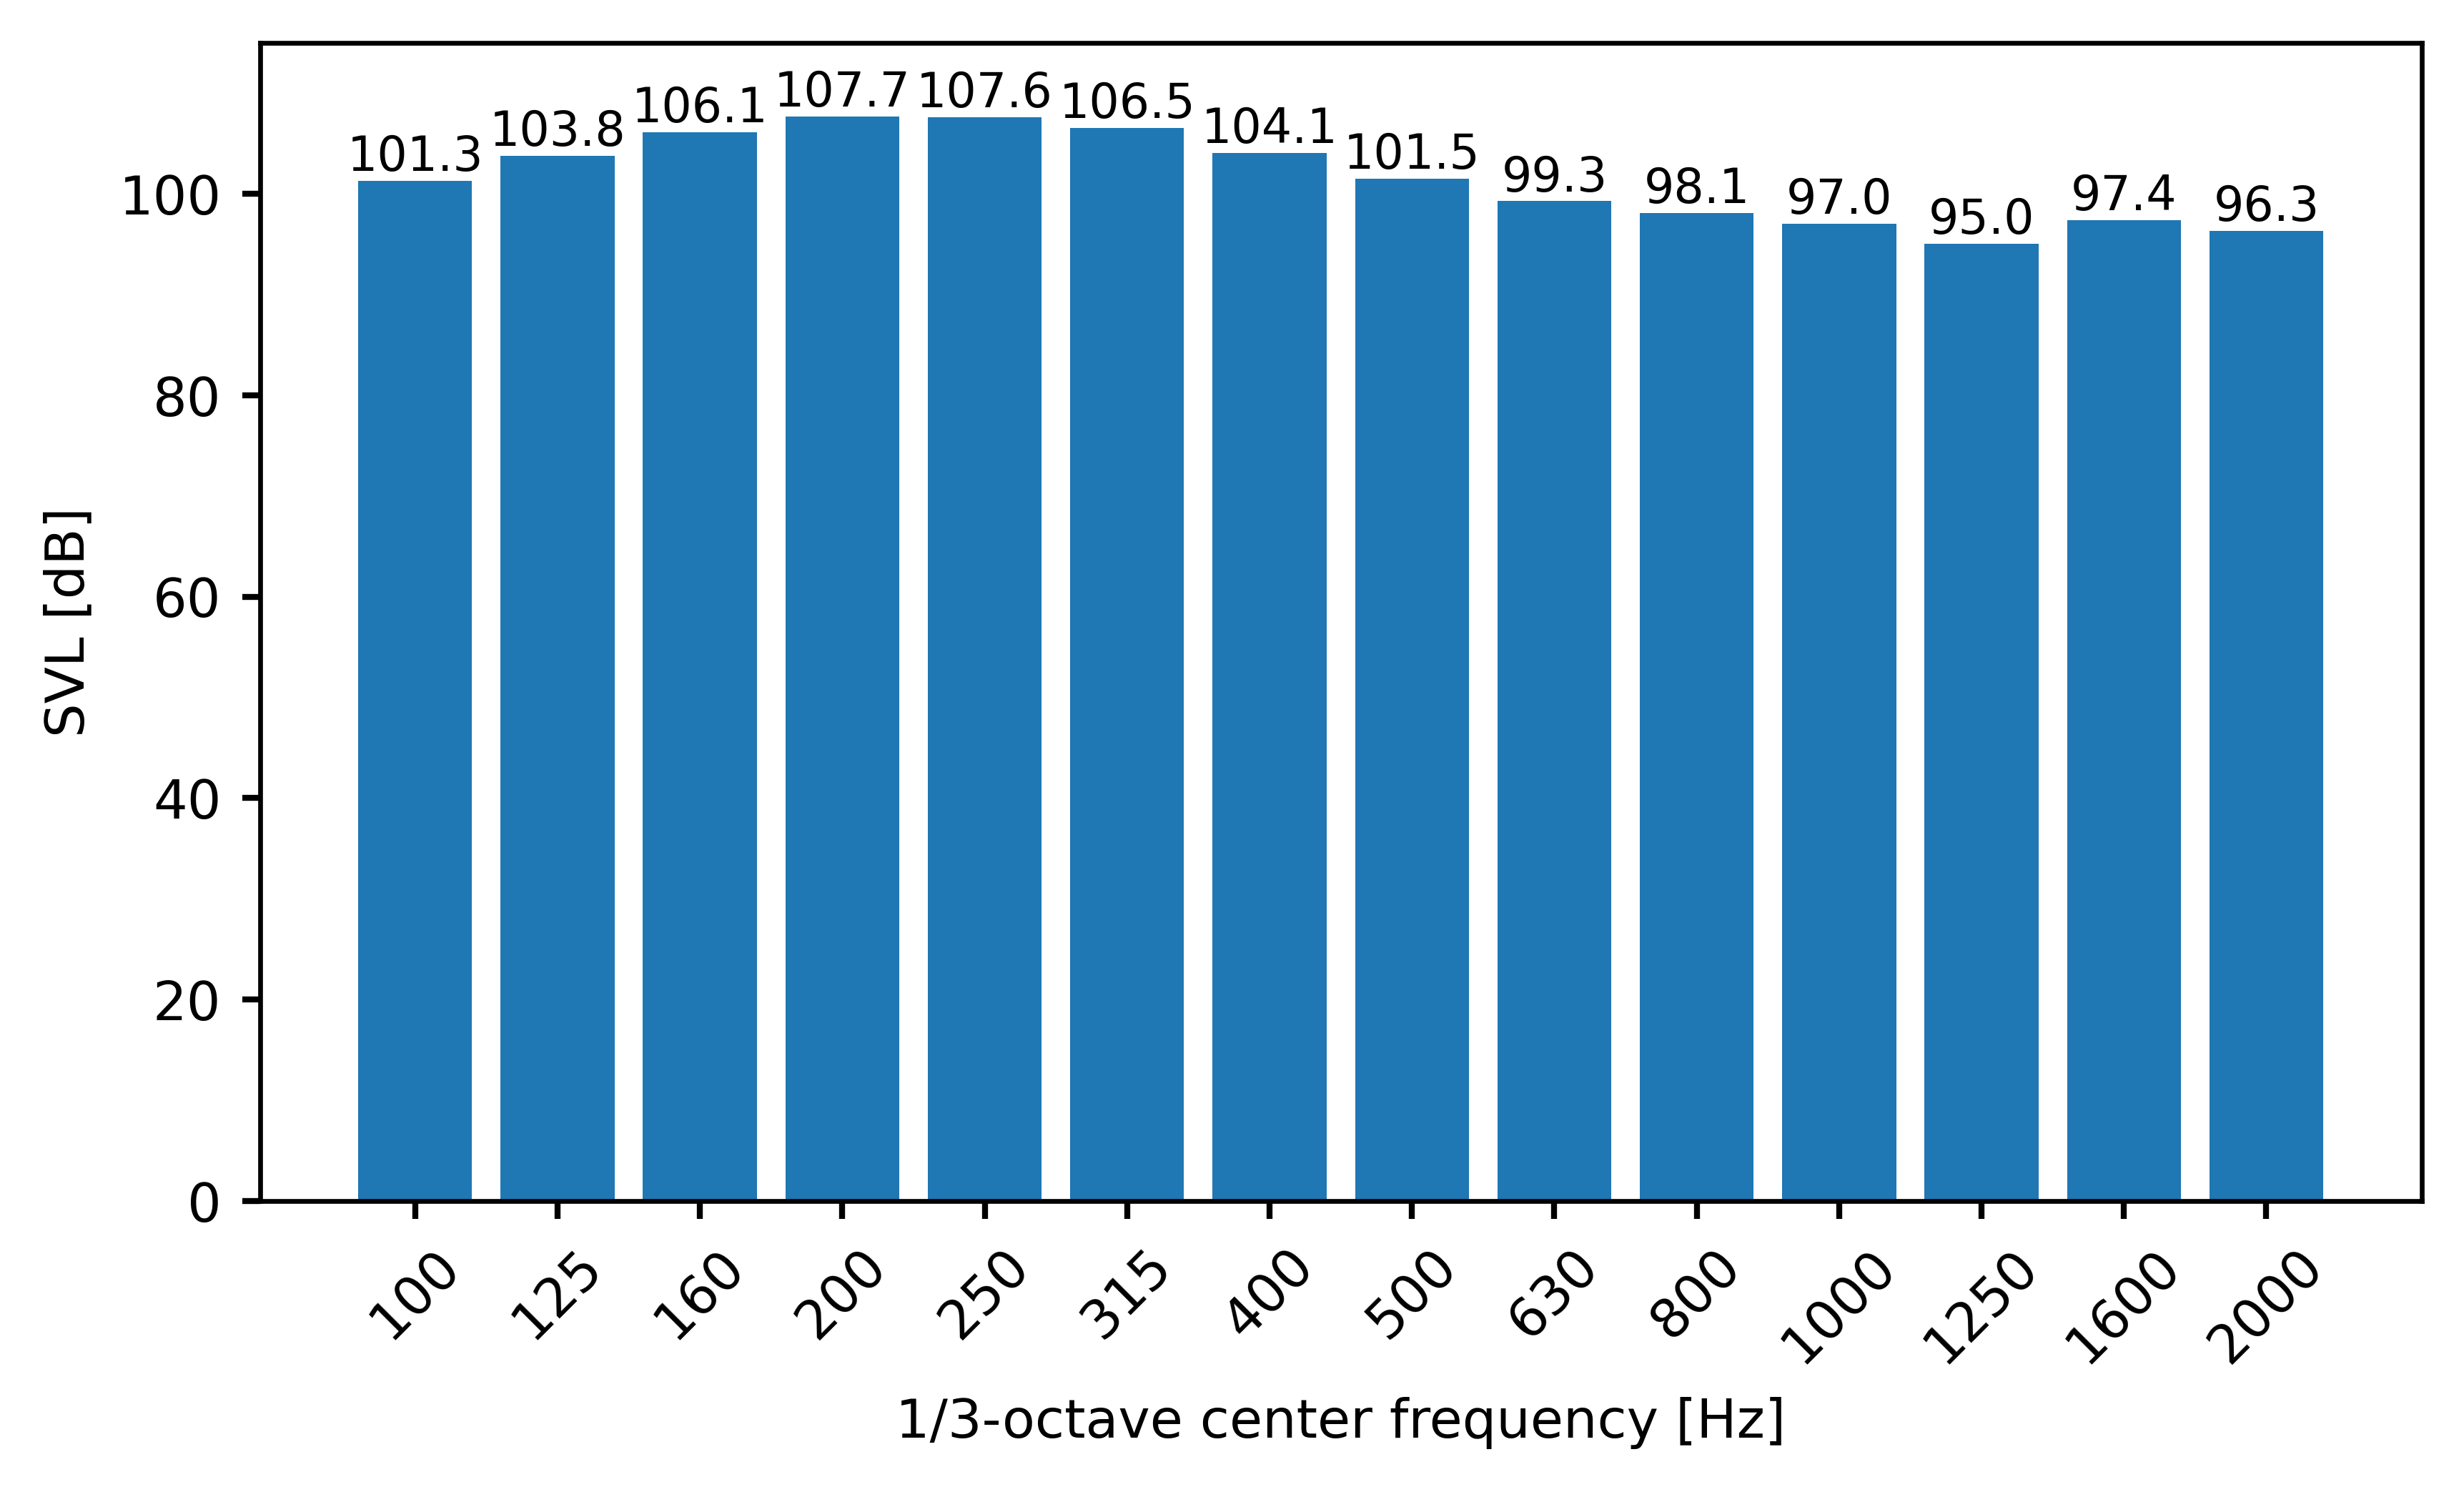
\includegraphics{fig/chap4/input_SVL.png}
	\caption{Input surface normal velocity in dB ref. $5\cdot10^{-8}\,\text{m/s}$, calculated using \ref{eq:input_velocity}}
\end{figure}

For the simulation, the sound power level of one single 1/3-octave band is divided into the 9 intermediate frequency steps by a 9.54 dB reduced sound power level for every single frequency within the band so that the sum of all frequencies results in the sound power level for the corresponding 1/3-octave band.




%\section{General simulation setup}

\section{Parametric study}
\label{section:parametric_study}
\subsection{Variation of underfloor geometry}

\begin{figure}[H]
	\centering
	\begin{subfigure}[b]{0.49\textwidth}
		\centering
		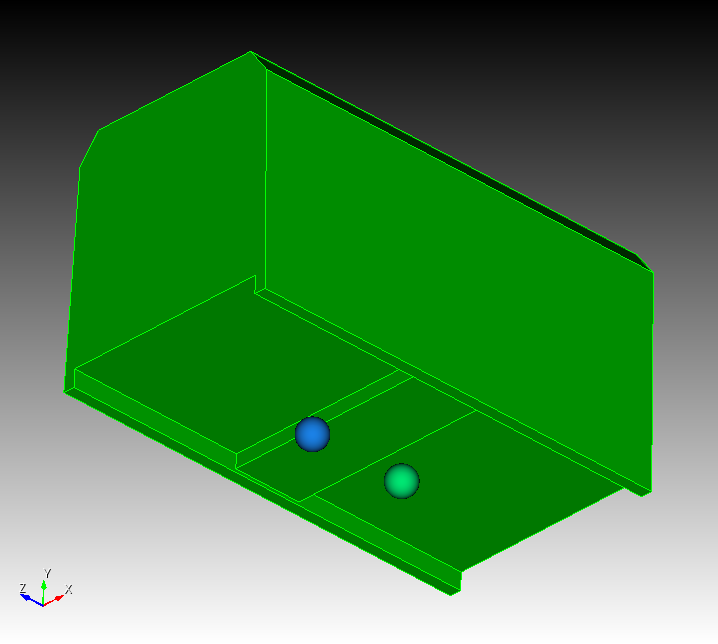
\includegraphics[width = 0.8\linewidth]{fig/chap4/geometry/no_underfloor_components_2.png}
		\caption{No underfloor components}
	\end{subfigure}
	\begin{subfigure}[b]{0.49\textwidth}
		\centering
		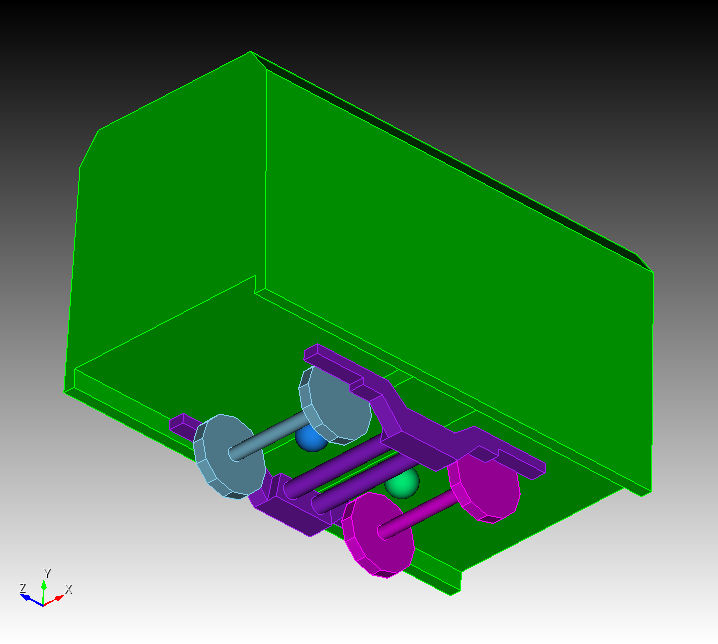
\includegraphics[width = 0.8\linewidth]{fig/chap4/geometry/no_air_suspension_2.png}
		\caption{No air suspension}
	\end{subfigure}
	\begin{subfigure}[b]{0.49\textwidth}
		\centering
		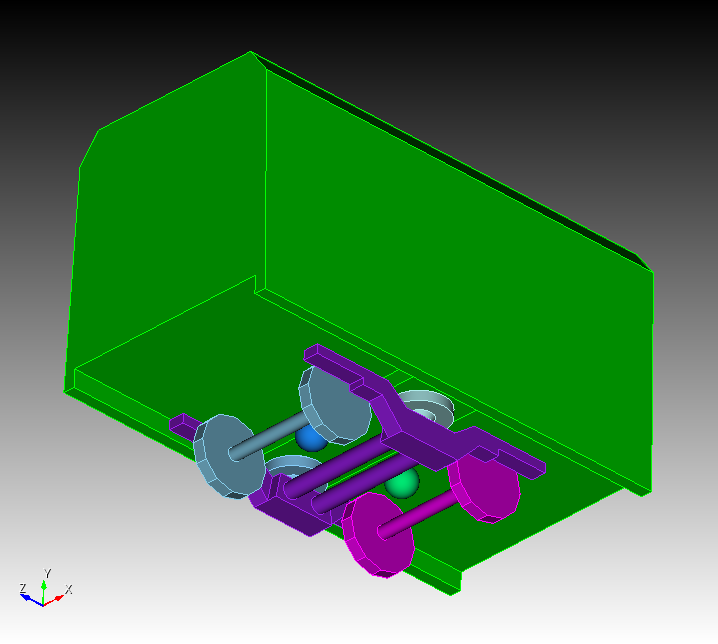
\includegraphics[width = 0.8\linewidth]{fig/chap4/geometry/initial_model_2.png}
		\caption{Initial model}
	\end{subfigure}
	\begin{subfigure}[b]{0.49\textwidth}
		\centering
		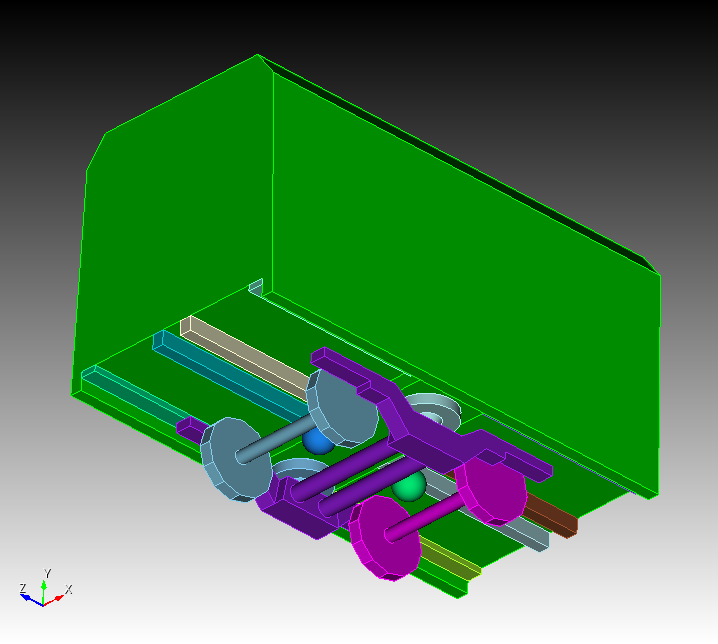
\includegraphics[width = 0.8\linewidth]{fig/chap4/geometry/additional_structures.png}
		\caption{Additional structures}
	\end{subfigure}

	\caption{Used geometry}
\end{figure}

\subsection{Inclusion of ground absorption}

In the finite element formulation, the ground absorption is modeled by the surface impedance boundary condition. The surface impedance is complex valued. The phase information of the surface impedance is lost when converting to absorption coefficient. For most of the time, (in acoustic data bank) only the absorption coefficient is provided but not the full impedance characteristic. To have an idea how the missing phase information of the impedance could affect the results. It assumed that the phase of the surface impedance are 0°, 30°, 45° and 60°.

In the initial simulation setup, the ground is modeled as a perfect reflecting plane. To have an idea how the unknown 

Due to a missing ground absorption measurement

\begin{figure}[H]
	\centering
	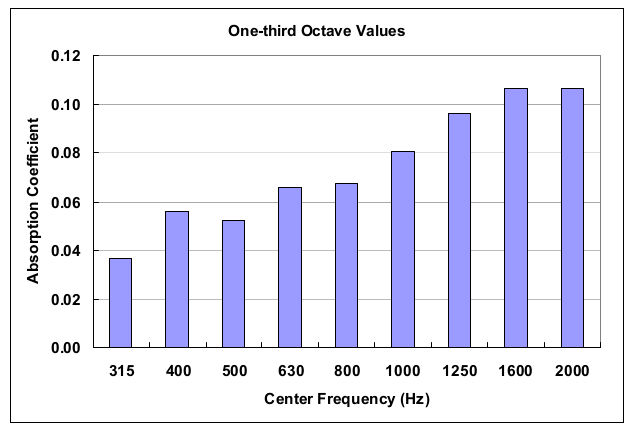
\includegraphics[width=0.7\textwidth]{fig/chap4/impedance/absorption_spectrum.png}
	\caption{Absorption coefficient in one-third octave bands \cite{Seybert2008MeasurementOP}}
	\label{fig:ground_absorption}
\end{figure}

\begin{table}[H]
	\caption{Estimated absorption coefficient from fig. \ref{fig:ground_absorption}, the values for frequency lower than 315 Hz are chosen arbitrary}
	\begin{tabular}{c|ccccccc}
		Freq (Hz)           & 100  & 125  & 160  & 200  & 250  & 315  & 400 \\ \hline
		$\alpha$ & 0.02 & 0.02 & 0.02 & 0.02 & 0.02 & 0.035 & 0.055
	\end{tabular}
	\newline
	\vspace*{10pt}
	\newline
	\begin{tabular}{c|ccccccc}
		Freq (Hz)  &  500  & 630  & 800  & 1000 & 1250 & 1600 & 2000 \\ \hline
		$\alpha$ & 0.05 & 0.065 & 0.065 & 0.08 & 0.095 & 0.105 & 0.105
	\end{tabular}
\end{table}

\begin{equation}
	\alpha = 1 - |R^2|
\end{equation}

\begin{equation}
	R = \frac{Z_s - Z_0}{Z_s + Z_0} = \frac{\frac{Z_s}{Z_0} - 1}{\frac{Z_s}{Z_0} + 1}
\end{equation}

\begin{equation}
	\tilde{Z_s} = \frac{Z_s}{Z_0} = \tilde{R_s} + j\tilde{X_s}
\end{equation}



\begin{equation}
	\begin{cases}
		\frac{4\tilde{R_s}}{\tilde{R_s}^2+\tilde{X_s}^2 + 2\tilde{R_s} + 1} = \alpha\\
		\arctan{\frac{\tilde{X_s}}{\tilde{R_s}}} = \varphi
	\end{cases}	
	\label{eq:impedance}
\end{equation}


\begin{figure}[H]
	\centering
	\begin{subfigure}[b]{0.8\textwidth}
		\centering
		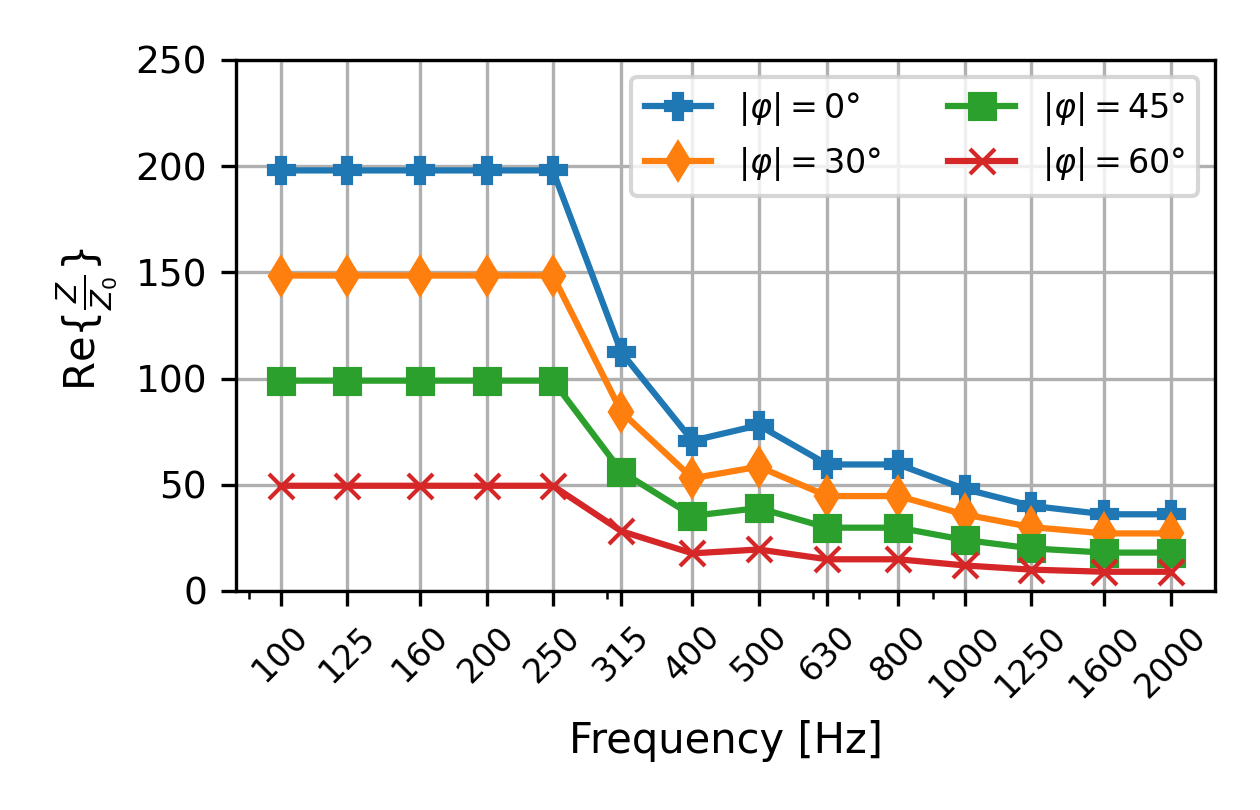
\includegraphics{fig/chap4/impedance/impedance_real.png}
	\end{subfigure}
	\begin{subfigure}[b]{0.8\textwidth}
		\centering
		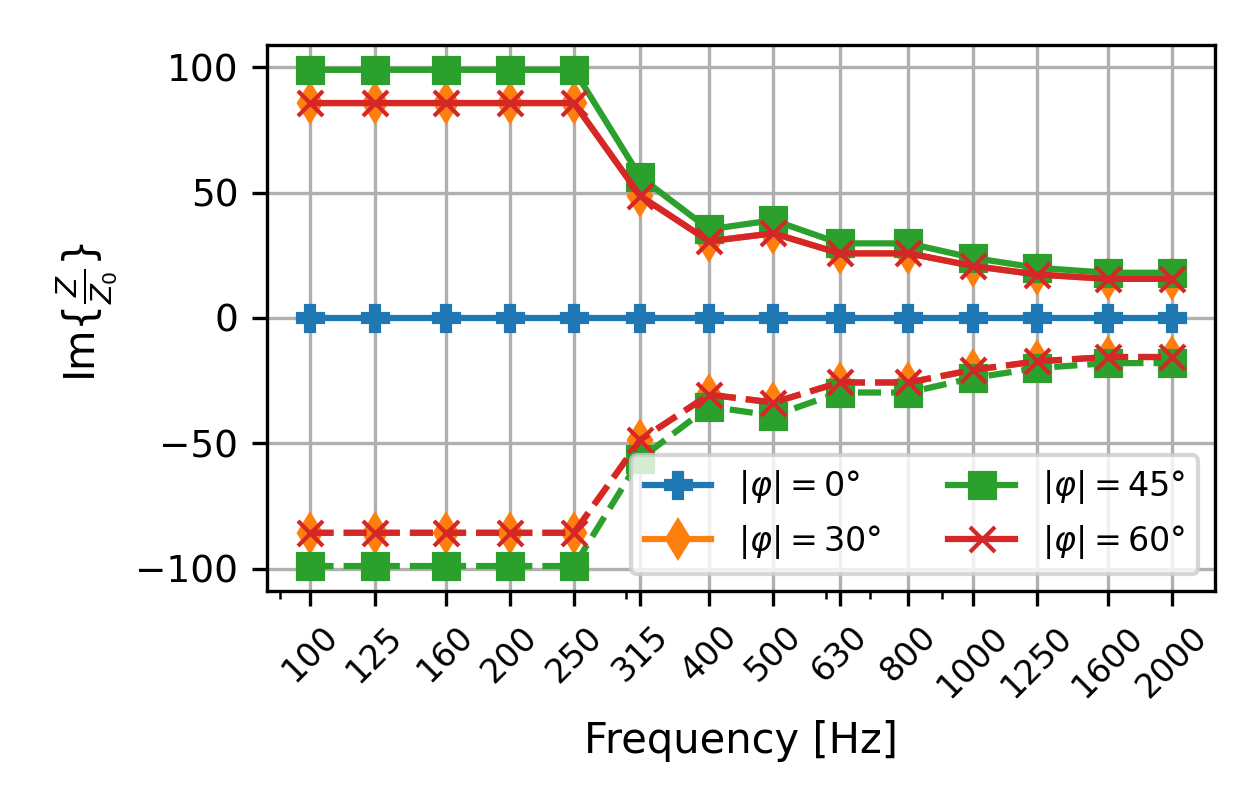
\includegraphics{fig/chap4/impedance/impedance_imag.png}
	\end{subfigure}
	\caption{Input surface impedance in one-third octave bands calculated using (\ref{eq:impedance})}
\end{figure}


\subsection{Variation of frequency steps per 1/3-octave band}